\chapter{Revisão da Literatura}
\label{cap2_revisao}

A revisão da literatura envolve a análise dos trabalhos precedentes que trataram o tema proposto, delineando o arcabouço conceitual dos aspectos a serem investigados pela pesquisa. Deve mostrar que o autor conhece parte da bibliografia (do assunto que será analisado) que determinou a seleção e a viabilidade do tema. A revisão da literatura apresenta citações diretas e indiretas dos autores consultados.

%-----------------------------------
\section{Citações: ABNT NBR 10520:2023}

Para os efeitos da norma, aplicam-se as seguintes definições:

\begin{alineas}
	\item citação: menção de uma informação extraída de outra fonte;
	\item citação de citação: citação direta ou indireta de um texto em que não se teve acesso ao original;
	\item citação direta: transcrição textual de parte da obra do autor consultado;
	\item citação indireta: texto baseado na obra do autor consultado.
\end{alineas}

%-----------------------------------
\subsection{Regras gerais de apresentação}

Na versão de 2023 da norma, as chamadas pelo sobrenome do autor, pela instituição responsável ou pelo título devem ser grafadas em letras maiúsculas e minúsculas, tanto no corpo da sentença quanto entre parênteses. A versão de 2002 exigia letras maiúsculas dentro dos parênteses, e esse ainda é o comportamento padrão do pacote \texttt{abntex2cite}. Confirme com o orientador qual versão da norma o curso adota. Exemplos:

\begin{enumerate}
	\item O aprendizado profundo (\textit{deep learning}) é, segundo \citeonline{Lecun2015DeepLearning}, um subcampo do aprendizado de máquina que tenta aprender abstrações por meio de múltiplos níveis de representação, obtidos pela composição de módulos não lineares simples.
	\item A diversidade pode ser alcançada usando conjuntos de treinamento diferentes, métodos iguais com diferentes hiperparâmetros ou métodos diferentes para cada modelo \cite{Polikar2012EnsembleLearning}.
\end{enumerate}

Nas citações diretas, deve-se especificar a(s) página(s), volume(s), tomo(s) ou seção(ões) da fonte consultada. Esses dados devem seguir a data, separados por vírgula e precedidos pelo termo que os caracteriza, de forma abreviada. Nas citações indiretas, a indicação da(s) página(s) consultada(s) é opcional.

As citações diretas de até três linhas devem estar contidas entre aspas duplas. As aspas simples são utilizadas para indicar citação no interior da citação. Exemplos (trechos ilustrativos; ajuste o texto e a página à fonte real):

\begin{enumerate}
	\item O aprendizado profundo (\textit{deep learning}) é, segundo \citeonline[p.~436]{Lecun2015DeepLearning}, \enquote{um subcampo do aprendizado de máquina que tenta aprender abstrações através de múltiplos níveis de representação}.
	\item \enquote{A diversidade pode ser alcançada usando conjuntos de treinamento diferentes, ou métodos iguais com diferentes hiperparâmetros ou métodos diferentes para cada modelo} \cite[p.~2]{Polikar2012EnsembleLearning}.
\end{enumerate}

As citações diretas com mais de três linhas devem ser destacadas com recuo de 4~cm da margem esquerda, com letra menor que a do texto e sem aspas.

\begin{citacao}
For example, if the probability of an event is not known with precision, then it may be characterized linguistically as, say, quite likely, not very unlikely, highly unlikely, etc., where quite likely, not very unlikely and highly unlikely are interpreted as labels of fuzzy subsets of the unit interval. Such subsets may be likened to ball-parks without sharply defined boundaries which serve to provide an approximate rather than exact characterization of the value of a variable \cite[p.~202]{zadeh1976fuzzy}.
\end{citacao}

%-----------------------------------
\section{Notas de rodapé e links}

Isso é uma nota de rodapé.\footnote{Texto da nota de rodapé.}

Mais informações sobre o pacote abnTeX2 podem ser encontradas em sua página no CTAN \cite{abntex2ctan}, disponível em \url{https://ctan.org/pkg/abntex2}.

Também é possível criar um link com texto, como na documentação do pacote \href{https://ctan.org/pkg/abntex2}{abnTeX2}.

%-----------------------------------
\section{Equações}

Equações simples podem ser descritas dentro das frases ou separadamente. Veja os dois exemplos.

A equivalência massa-energia é descrita pela famosa equação $ E = mc^2 $, proposta em 1905 por Albert Einstein.
Em unidades naturais ($ c = 1 $), a fórmula se reduz à identidade apresentada na Equação~\eqref{eq_massenergy}.

\begin{equation}
	E = m
	\label{eq_massenergy}
\end{equation}

Use ferramentas para auxiliar na criação de equações, como o \href{https://www.codecogs.com/latex/eqneditor.php?lang=pt-br}{CodeCogs}. Outro exemplo é a Equação~\eqref{eq_exemplo}.

\begin{equation}
	F(x) = \int_{x^{-1}}^{x^2} t \, dt
	\label{eq_exemplo}
\end{equation}

%-----------------------------------
\section{Figuras}

A Figura~\ref{fig_gatofofo} é apenas um exemplo de inserção de imagem. Você pode usar os formatos PNG, JPG ou PDF. Observe que o título da figura fica acima dela e a fonte, abaixo, conforme a NBR 14724. Toda ilustração deve indicar sua fonte, mesmo quando produzida pelo próprio autor. Use rótulos com nomes sugestivos para figuras, equações e tabelas, o que facilita a escrita do TCC. Não use imagens protegidas por direitos autorais sem autorização.

\begin{figure}[htb]
	\centering
	\caption{Gato fofo.}
	\label{fig_gatofofo}
	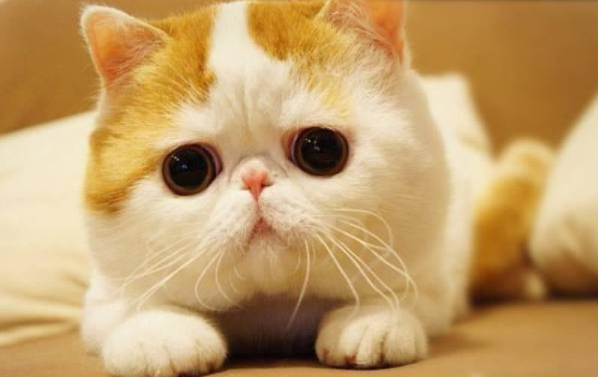
\includegraphics[width=0.5\textwidth]{Figuras/gatofofo.png}
	\fonte{Imagem ilustrativa (substitua pela fonte real da imagem).}
\end{figure}

Você também pode usar subfiguras para deixar o documento mais organizado. A Figura~\ref{fig_subfigname} ilustra um exemplo. Para citar uma subfigura específica, use \ref{subfig_cutecat} ou \ref{subfig_cutestdog}.

\begin{figure}[htb]
	\centering
	\caption{Animais de estimação fofos.}
	\label{fig_subfigname}
	\begin{subfigure}{0.3\textwidth}
		\centering
		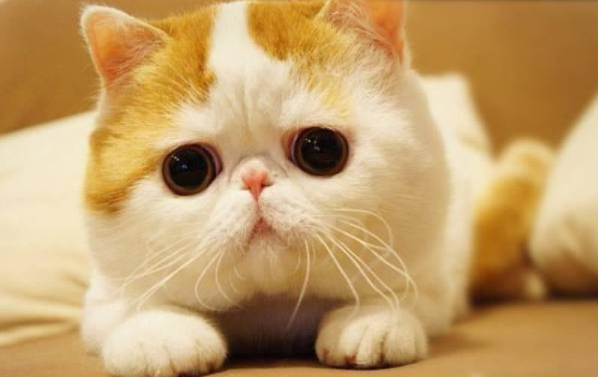
\includegraphics[width=\textwidth]{Figuras/gatofofo.png}
		\caption{Gato fofo.}
		\label{subfig_cutecat}
	\end{subfigure}\qquad
	\begin{subfigure}{0.3\textwidth}
		\centering
		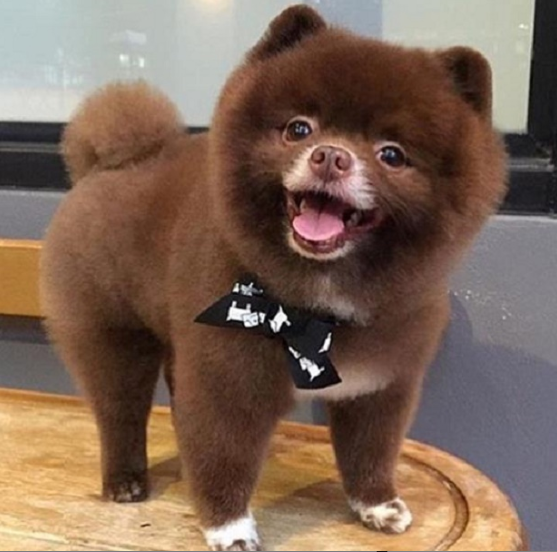
\includegraphics[width=\textwidth]{Figuras/cachorrofofo.png}
		\caption{Cachorro fofo.}
		\label{subfig_cutestdog}
	\end{subfigure}
	\fonte{Imagens ilustrativas (substitua pela fonte real das imagens).}
\end{figure}

%-----------------------------------
\section{Quadros: saídas, comandos e códigos}

Trechos de arquivos de configuração, saídas de comandos e códigos são conteúdo textual e devem ser apresentados como quadro, conforme o Quadro~\ref{qua_exemplocomando}.

\begin{quadro}[htb]
	\centering
	\caption{Listagem de arquivos gerados na compilação.}
	\label{qua_exemplocomando}
\begin{Verbatim}[fontsize=\small,frame=single]
$ ls main*
-rw-r--r--  1 autor users   3650 set 12 17:56 main.aux
-rw-r--r--  1 autor users   6366 set 12 17:43 main.bbl
-rw-r--r--  1 autor users    290 set 12 17:56 main.lof
-rw-r--r--  1 autor users  27937 set 12 17:56 main.log
-rw-r--r--  1 autor users    194 set 12 17:56 main.lot
-rw-r--r--  1 autor users    715 set 12 17:56 main.out
-rw-r--r--  1 autor users 159243 set 12 17:56 main.pdf
-rw-r--r--  1 autor users   4559 set 12 17:47 main.tex
-rw-r--r--  1 autor users    964 set 12 17:56 main.toc
\end{Verbatim}
%$ - esse comentário é para não confundir o realce de sintaxe do editor
	\fonte{Elaborado pelo autor.}
\end{quadro}

%-----------------------------------
\section{Tabelas}
\label{sec_tabelas}

A Tabela~\ref{tab_shorttable} apresenta o modelo de tabela que deve ser usado. Tabelas não têm bordas verticais nem fechamento lateral, e números devem manter a mesma quantidade de casas decimais, alinhados à direita; o texto deve ser alinhado à esquerda.

A ferramenta \texttt{Tables Generator}, disponível em \url{https://www.tablesgenerator.com/}, ajuda na construção de tabelas.

\begin{table}[htb]
	\centering
	\caption{Exemplo de tabela.}
	\label{tab_shorttable}
	\begin{tabular}{lrrr}
		\toprule
		Descrição    & \multicolumn{1}{c}{Valor 1} & \multicolumn{1}{c}{Valor 2} & \multicolumn{1}{c}{Valor 3} \\
		\midrule
		Aplicativo 1 & 1.352,70 &   1,22 &  1.358,00 \\
		Aplicativo 2 & 2.005,00 &  75,21 &  6.873,11 \\
		Aplicativo 3 & 8.648,00 &   5,45 &    852,00 \\
		Aplicativo 4 & 4.587,55 & 153,00 & 53.468,00 \\
		Aplicativo 5 &     0,00 &   0,00 &      0,00 \\
		\bottomrule
	\end{tabular}
	\fonte{Elaborado pelo autor.}
\end{table}

Para fazer referência a elementos que estão no apêndice, use: Tabela~\ref{tab_longtable} (Apêndice~\ref{apendiceA}).

Para fazer referência a elementos que estão no anexo, use: Anexo~\ref{anexoA}.

%-----------------------------------
\section{Algoritmos}
\label{sec_algoritmos}

O Algoritmo~\ref{alg:1} apresenta o pseudocódigo desenvolvido.

\begin{algorithm}[H]
	\SetAlgoLined
	\KwResult{Escreva aqui o resultado}
	inicialização\;
	\While{condição}{
		instruções\;
		\eIf{condição}{
			instrução1\;
			instrução2\;
		}{
			instrução3\;
		}
	}
	\caption{Como escrever algoritmos}
	\label{alg:1}
\end{algorithm}
